\section{Potential and actual infinity}

The work of \textcite{Lak00} provides a wide range of examples of
metaphorical reasoning in mathematics, while stressing the embodied
cognition involved in basic mathematical experience.  Some of
the ideas have been reworked by the authors, increasing the emphasis on
conceptual blending as central.  In particular, the analysis of
mathematical infinity, given in metaphorical form as the ``Basic Metaphor
of Infinity'' (BMI) in \textcite{Lak00}, is represented in blend form
in \textcite{nunez05} as the ``Basic Mapping of Infinity'' (so, still ``BMI'').

We show here how this blend works out in our setting.

\begin{figure}[h]
  \centering
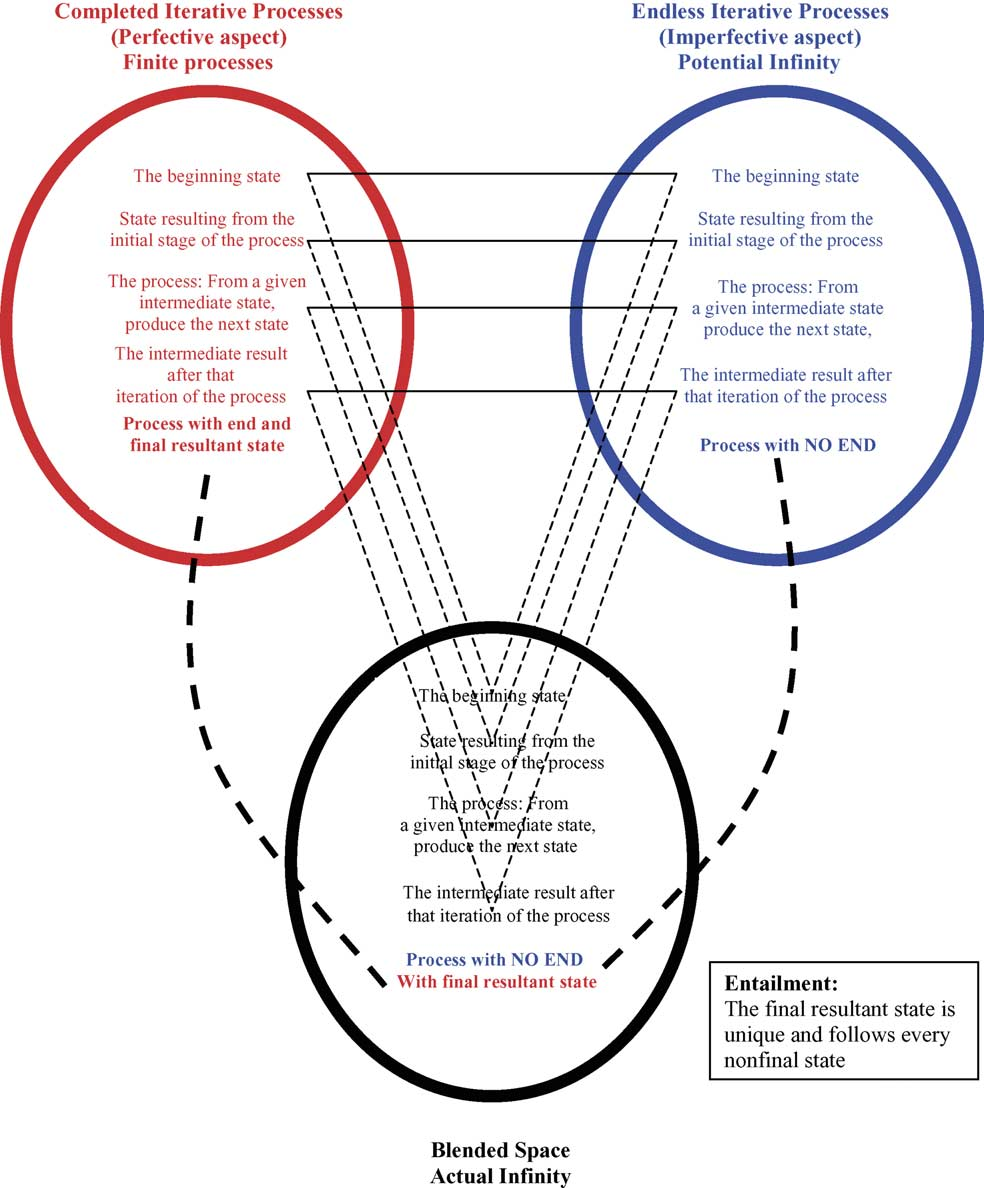
\includegraphics[width=0.4\textwidth]{transfin_nunez}  
  \caption{Blend from \textcite[p ??]{nunez05}}
  \label{fig:nunez_transfin}
\end{figure}

Figure~\ref{fig:nunez_transfin} gives an indication of the components
of the blend:
\begin{itemize}
\item The two input spaces at the top correspond to notions
of processes involving state change:
\begin{itemize}
\item  Completed Iterative Processes
are those that from some initial state, terminate in a final state
after a finite number of state transitions;
\item 
Endless Iterative Processes are those that continue indefinitely
to change state.
\end{itemize}
The marked correlations between features of the input spaces
indicate the common structure that is captured in our approach
by hte Generic Space, and as a result appear in the blend space.
\item 
Finally, the blend includes new features taken from both of the
input spaces, namely both ``process with no end'' and 
``final resultant state''.
\end{itemize}


%%% Local Variables: 
%%% mode: latex
%%% TeX-master: "mathsICCC"
%%% End: 
